\hypertarget{haskell}{%
\section{Haskell - Higher-Order Functions}\label{haskell}}

Haskell functions can take functions as parameters and return functions as return values. A function that does either of those is called a higher order function.


\hypertarget{curried-functions}{%
\subsection{Curried Functions}\label{curried-functions}}

Functions with multiple arguments are also possible by returning
functions as results. Functions that take their arguments one at a time
are called \textbf{curried functions}.

\begin{lstlisting}[language=Haskell]
ghci> max 4 5  
5 
max :: (Ord a) => a -> a -> a
-- Can also be written like: max :: (Ord a) => a -> (a -> a)

multThree :: (Num a) => a -> a -> a -> a  
multThree x y z = x * y * z
\end{lstlisting}

Curried functions are more flexible than functions on tuples, because
useful functions can often be made by partially applying a curried
function.

\hypertarget{currying-conventions}{%
\subsubsection{Currying Conventions}\label{currying-conventions}}

\begin{enumerate}
\def\labelenumi{\arabic{enumi}.}
\tightlist
\item
  The arrow -\textgreater{} associates to the right.
\item
  As a consequence, it is then natural for function application to
  associate to the left
\end{enumerate}

\begin{tcolorbox}[colback=red!5!white,colframe=red!75!black]
Unless tupling is explicitly required, all functions in Haskell are normally defined in curried form.
\end{tcolorbox}

\subsubsection{Currying infix functions}

Infix functions can also be partially applied by using sections. To section an infix function, simply surround it with parentheses and only supply a parameter on one side. That creates a function that takes one parameter and then applies it to the side that's missing an operand.

\begin{lstlisting}[language=Haskell]
ghci> max 4 5  
5 
max :: (Ord a) => a -> a -> a
-- Can also be written like: max :: (Ord a) => a -> (a -> a)

multThree :: (Num a) => a -> a -> a -> a  
multThree x y z = x * y * z
\end{lstlisting}

\clearpage
\subsection{Higher-Order function declaration}

\begin{lstlisting}[language=Haskell]
applyTwice :: (a -> a) -> a -> a  
applyTwice f x = f (f x)  
\end{lstlisting}

Before, we didn't need parentheses because -> is naturally right-associative. However, here, they're mandatory. They indicate that the first parameter is a function that takes something and returns that same thing. The second parameter is something of that type also and the return value is also of the same type. We could read this type declaration in the curried way, but to save ourselves a headache, we'll just say that this function takes two parameters and returns one thing. The first parameter is a function (of type a -> a) and the second is that same a.

\begin{lstlisting}[language=Haskell]
zipWith' :: (a -> b -> c) -> [a] -> [b] -> [c]  
zipWith' _ [] _ = []  
zipWith' _ _ [] = []  
zipWith' f (x:xs) (y:ys) = f x y : zipWith' f xs ys  

ghci> zipWith' (+) [4,2,5,6] [2,6,2,3]  
[6,8,7,9]  
\end{lstlisting}

The function zipWith' takes a function and two lists as parameters and then joins the two lists by applying the function between corresponding elements.

\hypertarget{map-function}{%
\subsection{Map Function}\label{map-function}}

The higher-order library function called map applies a function to every
element of a list.

\begin{lstlisting}[language=Haskell]
map :: (a -> b) -> [a] -> [b]

> map (+1) [1,3,5,7]
[2,4,6,8]
\end{lstlisting}

\hypertarget{filter-function}{%
\subsection{Filter Function}\label{filter-function}}

The higher-order library function filter selects every element from a
list that satisfies a predicate.

\begin{lstlisting}[language=Haskell]
filter :: (a -> Bool) -> [a] -> [a]

> filter even [1..10]
[2,4,6,8,10]
\end{lstlisting}

\clearpage
\hypertarget{foldr-function-folg-right}{%
\subsection{Foldr Function (Folg
right)}\label{foldr-function-folg-right}}

\begin{lstlisting}[language=Haskell]
f [] = v  //Neutral Element
f (x:xs) = x $\oplus$ f xs
\end{lstlisting}

f maps the empty list to some value v (Default value), and any non-empty
list to some function $\oplus$  applied to its head and f of its tail.

\begin{lstlisting}[language=Haskell]
//Example
sum = foldr (+) 0
\end{lstlisting}

\begin{figure}[H]
\centering
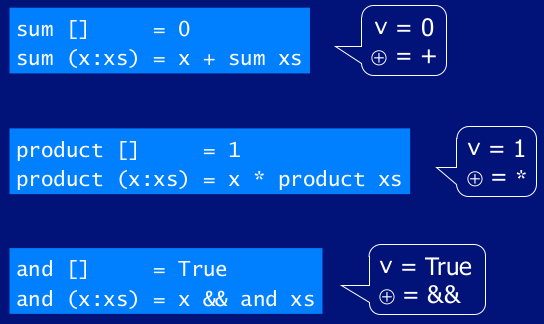
\includegraphics[width=0.5\textwidth]{figures/fold_examples.png}
\caption{Foldr examples}
\end{figure}

\begin{figure}[H]
\centering
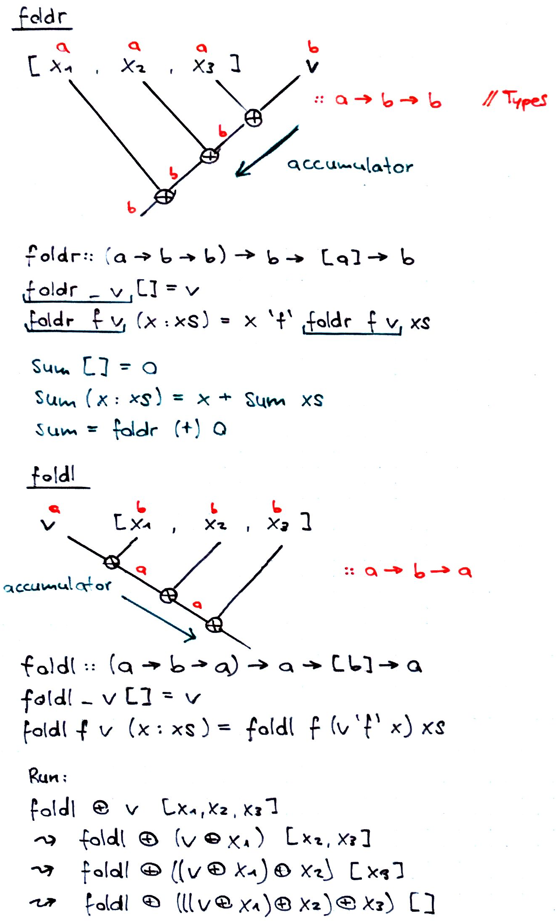
\includegraphics[width=0.7\textwidth]{figures/foldr.png}
\caption{Foldr}
\end{figure}

\hypertarget{other-library-functions}{%
\subsection{Other Library Functions}\label{other-library-functions}}

The library function (.) returns the composition of two functions as a
single function.

\begin{lstlisting}[language=Haskell]
(.) :: (b -> c) -> (a -> b) -> (a -> c)
f . g = $\lambda$x -> f (g x)

example:
odd :: Int -> Bool
odd = not . even
\end{lstlisting}

\hypertarget{all}{%
\subsubsection{all}\label{all}}

The library function all decides if every element of a list satisfies a
given predicate.

\begin{lstlisting}[language=Haskell]
> all even [2,4,6,8,10]
True
\end{lstlisting}

\hypertarget{any}{%
\subsubsection{any}\label{any}}

Dually, the library function any decides if at least one element of a
list satisfies a predicate.

\begin{lstlisting}[language=Haskell]
> any (== ' ') "abc def"
True
\end{lstlisting}

\hypertarget{takewhile}{%
\subsubsection{takeWhile}\label{takewhile}}

The library function takeWhile selects elements from a list while a
predicate holds of all the elements.

\begin{lstlisting}[language=Haskell]
> takeWhile (/= ' ') "abc def"
"abc"
\end{lstlisting}


\clearpage